\documentclass[a4paper]{article}
\usepackage{fullpage}
\usepackage{amsmath}
\usepackage{graphicx}
\usepackage[colorlinks]{hyperref}

\newcommand{\dd}{\text{d}}
\newcommand{\ii}{\text{i}}

\newcommand{\of}[1]{\left( {#1} \right)}
\newcommand{\fracd}[2]{\frac{\dd{}{#1}}{\dd{}{#2}}}

\newcommand{\dhref}[1]{\href{#1}{#1}}
\newcommand{\mailhref}[1]{\href{mailto:#1}{#1}}

\title{Final report on ``Heterogeneity of the Suprachiasmatic
Nucleus'' {\em BO 3612/2-1}}
\author{Hanspeter Herzel  \mailhref{h.herzel@biologie.hu-berlin.de},\\
        Grigory Bordyugov \mailhref{grigory.bordyugov@gmail.com}}
\date{\today}

\begin{document}
\maketitle

\thispagestyle{empty}

\begin{abstract}
  This DFG-supported project was aiming at uncovering the rhythmic
  properties of circadian oscillator arrays of the SCN on different
  scales, ranging from single cell oscillations to ensemble effects on
  the tissue level. We report advances on several levels, including
  the conceptual (phase of entrainment), single-cell mechanistic
  (molecular workings of regulatory gene networks), and tissue-wide
  (dynamics of oscillator ensembles). The common pattern appearing
  here is that a substantial number of circadian phenomena can be well
  understood in the framework of relatively simple mathematical
  models, parameterized by few parameters such as amplitude, period
  and phase of oscillations. Additionally, the collaboration with the
  lab of Prof Toru Takumi in RIKEN resulted in discovery of Choroid
  Plexus as another strong circadian oscillator in brain with the
  rhythmicity levels comparable or even exceeding those of the SCN.
\end{abstract}

%% \tableofcontents

\newpage

\section{Overview / Zusammenfassung}
The main project aims were to understand the generation and
coordination of circadian rhythms in the mammalian SCN on different
scales which can range from the single cell periodicity to the
coordination of oscillations on the level of the whole organ. We are
glad to be able to report advances on at least three different levels
of this hierarchy.

On a single cell level, we present a computational framework for
mechanism-focused modeling of gene regulatory networks. Using a very
simple and intuitive description of the interaction between genes
together with their regulatory elements, the framework allows to
define interactions between the chosen genes and automatically tune
the parameters of the model, aiming at fitting a chosen set of
experimental data.  Whereas we have achieved a remarkable degree of
agreement between the simulated oscillations and their experimental
counterpart, the question of the uniqueness of the parameter values in
the model is still open and requires further investigations.

If one chooses to abstract away the details of how rhythms generated,
be it on the single cell or the organism level, and is only interested
in few fundamental oscillation properties such as amplitude, period
and the of the oscillations, the simplest mathematical oscillator
models turn out to be a great predictor for a substantial variety of
observed phenomena. In this project, we continued our previous efforts
to understand and describe the behaviour of entrainment phase under
different conditions. Our main contribution here is a new conceptual
treatment of photoperiod and its influence on entrainment phase. We
have discovered the ``entrainment onion'' \--- the counterpart of the
Arnold tongue under varying photoperiod (instead of Zeitgeber
strength) and showed that changes in photoperiod can effectuate
significantly larger deviations of entrainment phase.

Considering the SCN as an ensemble of interacting circadian neurons,
we proposed to use a new measure for its synchronization property -
the Moran's I statistics, previously nearly unknown on the field of
chronobiology. This statistics complements the more traditional
Kuramoto's order parameter in being sensitive not only to the global
distribution of the phases, but rather to how well neighbouring
oscillators are correlated. With the help of Moran's I, it became
possible to automatically classify between regimes in the SCN that
would have remained undistinguishable using Kuramoto's order parameter
only.

In conclusion, we report on the discovery of the extremely strong
rhythmicity in the choroid plexus (CP) (experiments performed in the
lab of Prof Toru Takumi). CP seems to be at least as robust an
oscillator as the SCN, having a higher amplitude of circadian
oscillations and a slightly shorter period. We proposed that the
remarkable rhythmic properties of the CP can be modelled by
oscillators with the so-called ``twist'', i.e. dependence of the
instantaneous period on the amplitude. Co-culture experiments with the
SCN and CP additionally suggest that the CP can tune the oscillations
in the SCN.


\newpage

\section{Main results: From modeling of single neuron oscillations to
ensembles dynamics of the SCN tissue}
Due to the space constraints for the report, below we are presenting
the most exciting (from our point of view) results obtaining during
the running time of project. A full list of publications and
manuscripts in review is given in the ``Formal'' section.

We start by discussing results on conceptual modeling of entrainment
phases in single oscillators (which can be though as an abstraction of
single cells or organisms, depending on the larger view), then present
our advances on mechanistic modelling of gene regulatory networks that
produce circadian oscillations in single cells, and look at a new
statistics that helps to characterize spatial synchronization of
rhythmic neurons on the tissue level in the SCN. We conclude by a
short report on discovering the choroid plexus as an extremely strong
circadian oscillator in the mammalian brain.


\subsection{Circadian entrainment phase: Towards a simple mathematical
model}


\subsection{Semi-automatic modeling for gene regulatory networks}
Within his masters dissertation, Matthew
Kondoff~\cite{kondoff2015modeling} looked at a way of automatically
generating computational models from human-readable description of
regulatory gene networks. His efforts resulted in an R package, with
the help of which a convenient way of numerical modeling was
providing, thus hiding the low-level nitty-gritty of translating the
network description into formulas and computer code.

\begin{figure}
\begin{center}
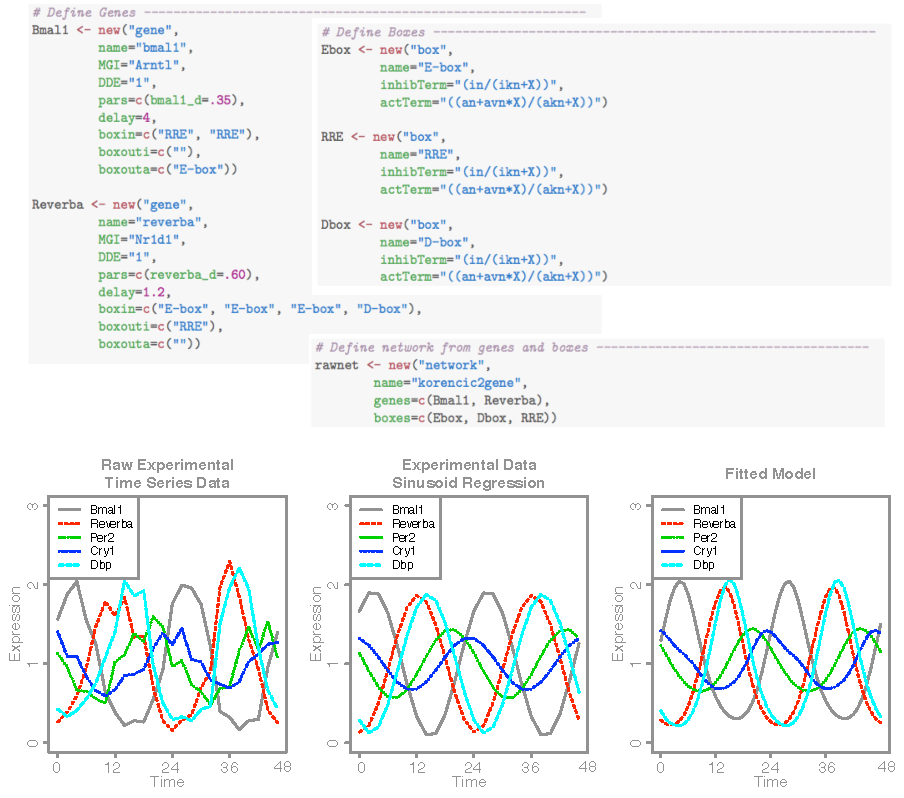
\includegraphics[width=\linewidth]{figures/matt/matt.pdf}
\end{center}
\caption{
  {\bf Upper panel} An example of a human-readable description of a
  gene regulatory network consisting of two genes (Bmal1 and
  Reverb$\alpha$) and three boxes (Ebox, RRE, Dbox).
  {\bf Lower panel} Comparison between oscillations in microarray
  data, the extracted first harmonic and the fit by a model with five
  genes.
\label{fig::matt}
}
\end{figure}

An example description of a simple two-gene, three-box network is
represented in Figure \ref{fig:matt}, upper panel. A highly
human-readable source code in R programming language automatically
produces then an optimized numerical simulation framework with
underlying low-level code for the nonlinear equations in C language
(for performance reasons). As a next step, the unknown parameters of
those nonlinear equations are found to fit the simulated oscillations
(Figure \ref{fig::matt}, lower panel, right plot) to given
experimental data (Figure \ref{fig::matt}, lower panel, left plot).
The data used here came from~\cite{zhang2014circadian}, being a set of
24 microarray assays collected in two hours intervals, totalling 48
hours worth of time series length. Before fitting, the parameters of
the $~$24 hours harmonic were extracted from the data (period,
relative phases and relative amplitudes) and used to define the cost
function in the fitting procedure. For the optimization procedure, the
so-called particle swarm optimzation (see~\cite{zambrano2012hydropso})
was used with optimized initial conditions,
see~\cite{richards2004choosing}.


\subsection{Moran's I as a measure for spatial (in)homogeneity between
oscillating cells}

In mammals, the SCN seems to play the central role in coordinating the
circadian rhythms across the whole
organism~\cite{reppert2002coordination}. The SCN is a densely packed
brain region containing dozens of thousands of rhythmic neurons and
can be anatomically classified in several regions, depending on what
neurotransmitter the underlying neurons can secret and react to. The
dorsal and ventral parts of the SCN represents the most obviously
different parts of the whole organ~\cite{yamaguchi2003synchronization}
and show quite different rhythmical behaviour. In this subproject, we
aimed at quantifying the spatial inhomogeneities across SCN slices in
terms of their synchronization properties.

The standard way to quantify the degree of synchronization in an
ensemble of oscillators has traditionally been the Kuramoto order
parameter $R$~\cite{kuramoto2012chemical}. The idea behind can be
visualized by placing each of the interacting oscillators on a unit
circle according to the oscillator's instantaneous phase and
calculating the centroid of resulting distribution of oscillators. The
absolute value of $R$, i.e. the distance of the centroid from the
origin, would then show the degree of instantaneous synchronization.
If, for instance, all oscillators are (nearly) uniformly distributed
along the unit circle, their centroid would be very close to origin
and $R$ would be close to zero. On contrary, if most of the
oscillators are grouped around a preferred phase, the centroid would
be close to that point and its distance from the origin (the absolute
value of $R$) would be close to one.

\begin{figure}
\begin{center}
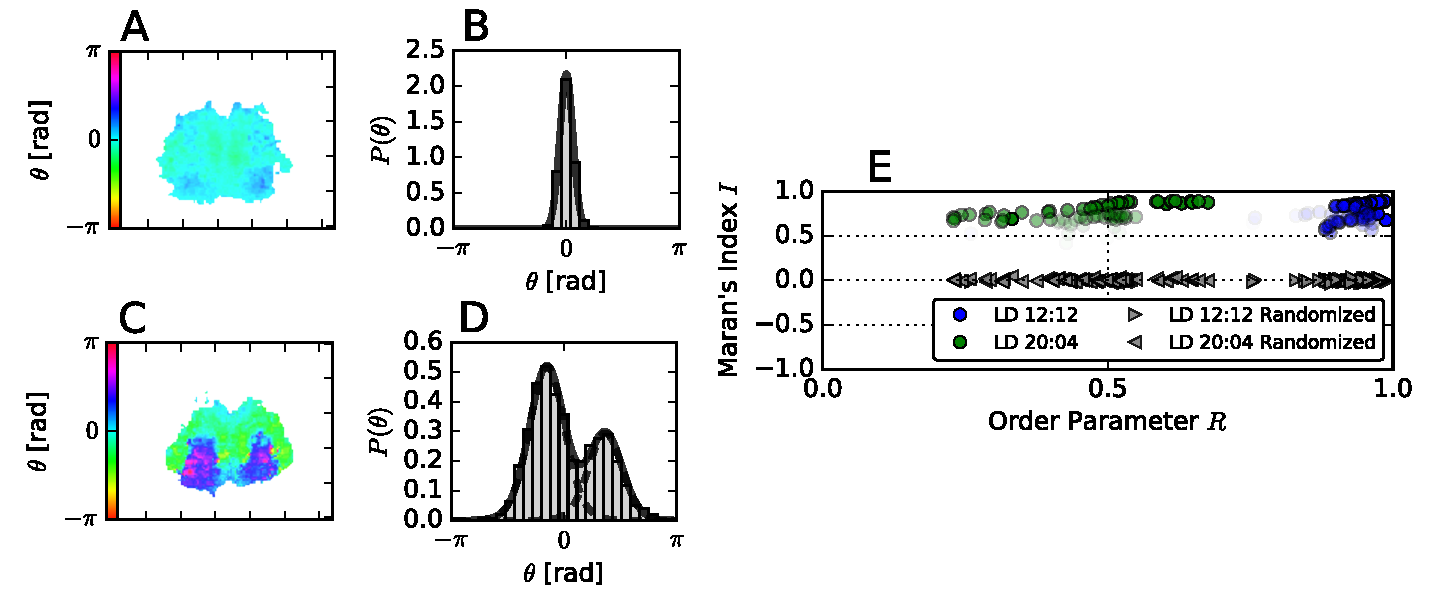
\includegraphics[width=\linewidth]{figures/mi/mi.pdf}
\end{center}
\caption{
  {\bf (A)} and {\bf (C)} Colour-coded distribution of oscillation
  phases of neurons across an SCN slice under equinox and long-day
  conditions, respectively.
  {\bf (B)} and {\bf (D)} The corresponding distributions of phases.
  {\bf (E)} Time traces in the coordinate plane of Kuramoto's order
  parameter $R$ and Moran's I.
\label{fig::mi}
}
\end{figure}

This approach, however, assumes no special arrangement between the
oscillating units, such as, for example, their ordering in space
relatively to each other. Looking for a better way to measure such
spatial aspect of synchronization across neurons, Dr Christoph Schmal
stumbled upon the so-called Moran's I statistics, which has been
widely used in geographical and sociological sciences for quantifying
the spatial correlation in units with a certain arrangement in
space~\cite{moran1950notes}. Moran's I takes into account the
arrangement of units in space by calculating the correlation between
the units weighted by the distance between them. So, for example, a
black and white chess board would corresponding to a Moran's I value
of $-1$, reflecting the largest possible anti-correlation between
neighbouring units and a nearly uniform homogeneous state would
correspond to the Moran's I value of 1 (the largest possible value).
Moran's I turned out to complement the traditional Kuramoto's order
parameter $R$ in a most insightful way when analyzing the rhythmicity
of neurons in SCN slices~\cite{schmal2017moran}. Figure~\ref{fig::mi}
from that paper shows two examples of phase distribution across SCN
slices (see (A) and (B) for colour-coded representations and (B) and
(D) for the probability distribution of phases).

When plotting the values of Moran's I vs Kuramoto's order parameter
$R$ (Figure~\ref{fig::mi} (E)), we have found scenarios with both
statistics giving complementary results. It is, for example, possible
that Moran's I remains close to zero, whereas the order parameter $R$
is non-zero. This situation would emerge when all neurons have phases
close to each other but the spatial correlation between neighbouring
neurons is absent. The opposite situation with relatively low values
of Kuramoto's order parameter $R$ and Moran's I close to one arises
when the spread of phases between the oscillators is large, but most
neighbours are relatively strongly correlated (green dots in
Figure~\ref{fig::mi} (E)). The influence of the photoperiod on the
observed interplay beween $R$ and Moran's I certainly deserves further
investigation, also in the light of the above discussion of the role
of photoperiod in entrainment phase.


\subsection{Robust circadian oscillations in the Choroid Plexus}

As the last piece of results within this project, we are reporting
here on the discovery of the Choroid Plexus (CP) as a extraordinary
robust circadian oscillator. By screening for periodic Bmal1-Eluc
expression across different brain regions, Dr Jihwan Myung found that
the periodicity of BMAL1 expression in the CP stood out among all
explants sampled~\cite{myung2017choroid}. The CP showed a remarkable
degree of phase synchrony on the single cell level, even beating that
of the SCN. Having assumed that the relative phasing of neurons across
the SCN can encode photoperiod, we speculated that the somewhat
simpler organization of the CP does not reflect such second-order
characteristics of circadian rhythmicity (such as, for instance, the
photoperiod) and hence adopts a less sophisticated, though stronger,
rhythmicity pattern.

The circadian oscillations in the CP were additionally modeled by the
so-called ``twist'' model. The twist represents the dependency of the
oscillator's period on its instantaneous amplitude. Such correlations
were found in the CP and the experimentally observed dependence of the
oscillation period on coupling, modulated by the gap junction blocker
meclofenamic acid (MFA), was successfully reproduced in a mathematical
model with twist. The main observed effect was the lengthening of the
oscillation period upon the application of MFA, which was mirrored by
the decreased coupling strength in the model.


\newpage

\section{Formal}

\subsection{Published and submitted manuscripts}
A total of 7 manuscripts have been enabled by this project, five of
them having already been published and two being under review:
\cite{bordyugov2015tuning,schmal2015theoretical,kondoff2015modeling,schmal2017moran,wagner2017plant,myung2017choroid,schmal2017measuring}


\subsection{Personnel}
For the duration of the project, Dr Christoph Schmal had the position
of post-doctoral researcher at the ITB Berlin, funded by this project.

\subsection{Cooperation activities between Berlin and Tokyo}

\subsubsection{Telecom conferences}
During the three years of the project, we maintained bi-weekly Skype
conferences to synchronize our activities between Tokyo and Berlin.

\subsubsection{Visits}
The following visits between Toru Takumi's Lab at RIKEN and the
Institute for Theoretical Biology in Berlin were possible through the
project:
\begin{itemize}
  \item[-] Pia Rose visited Riken from Marth 2nd through April 25th 2015,
  \item[-] Christoph Schmal visited Riken from June 18th through July 3rd
  2014,
  \item[-] Hanpspeter Herzel visited Riken from July 17th through July
  20th 2014,
  \item[-] Toru Takumi visited the ITB in Berlin on three occasions from
  2014 through 2016,
  \item[-] GB visited RIKEN from February 10th through March 1st 2014.
\end{itemize}

\subsection{Conferences}
The results of the research on the project were presented at the
Gordon Conference on Chronobiology (Newport, RI in summer 2013, also
first contact with Jihwan Myung established there), at the conference
of the Japanese Society for Mathematical Biology (Osaka, Summer 2014),
at the congress of European Biological Rhythms Society in M\&unchen
(Fall 2014), and at the meeting of SRBR (summer 2016).

\subsection{Student theses and projects}
We are reporting the following supervising activity, made possible
within this project:

Matthew Kondoff build a tool for automatically generating and
exploring regulatory networks of genes and fitted them to microarray
data of Hogenesch et al., which resulted in an R package
\cite{kondoff2015modeling}. Anna-Marie Finger and Lorena Sofia Lopez
Zepeda investigated the circadian regulation of immune system and
liver. Sungsoo Lim and Marta del Olmo conducted computer-assisted
studies of entrainment phase in several models of circadian clock.


\bibliographystyle{vancouver}
\bibliography{jg-report}
\end{document}
